\documentclass[12pt]{article}
\usepackage{lmodern}
\usepackage[margin=1in]{geometry}
\usepackage{float}
\usepackage{amssymb,amsmath}
\usepackage{multicol}
\usepackage{ifxetex,ifluatex}
\usepackage{fixltx2e} % provides \textsubscript
\ifnum 0\ifxetex 1\fi\ifluatex 1\fi=0 % if pdftex
  \usepackage[T1]{fontenc}
  \usepackage[utf8]{inputenc}
\else % if luatex or xelatex
  \ifxetex
    \usepackage{mathspec}
    \usepackage{xltxtra,xunicode}
  \else
    \usepackage{fontspec}
  \fi
  \defaultfontfeatures{Mapping=tex-text,Scale=MatchLowercase}
  \newcommand{\euro}{€}
\fi
% use upquote if available, for straight quotes in verbatim environments
\IfFileExists{upquote.sty}{\usepackage{upquote}}{}
% use microtype if available
\IfFileExists{microtype.sty}{%
\usepackage{microtype}
\UseMicrotypeSet[protrusion]{basicmath} % disable protrusion for tt fonts
}{}
\usepackage{graphicx}
\makeatletter
\def\maxwidth{\ifdim\Gin@nat@width>\linewidth\linewidth\else\Gin@nat@width\fi}
\def\maxheight{\ifdim\Gin@nat@height>\textheight\textheight\else\Gin@nat@height\fi}
\makeatother
% Scale images if necessary, so that they will not overflow the page
% margins by default, and it is still possible to overwrite the defaults
% using explicit options in \includegraphics[width=4in][width, height, ...]{}
\setkeys{Gin}{width=\maxwidth,height=\maxheight,keepaspectratio}
\ifxetex
  \usepackage[setpagesize=false, % page size defined by xetex
              unicode=false, % unicode breaks when used with xetex
              xetex]{hyperref}
\else
  \usepackage[unicode=true]{hyperref}
\fi
\hypersetup{breaklinks=true,
            bookmarks=true,
            pdfauthor={Brandon LeBeau},
            pdftitle={PSQF 4143: Section 2},
            colorlinks=true,
            citecolor=blue,
            urlcolor=blue,
            linkcolor=magenta,
            pdfborder={0 0 0}}
\urlstyle{same}  % don't use monospace font for urls
\setlength{\parindent}{0pt}
\setlength{\parskip}{6pt plus 2pt minus 1pt}
\setlength{\emergencystretch}{3em}  % prevent overfull lines
\setcounter{secnumdepth}{0}

\title{PSQF 4143: Section 2}
\author{Brandon LeBeau}
\date{}

\begin{document}
\maketitle

\section{Summarizing Data}\label{summarizing-data}

\begin{itemize}
\itemsep1pt\parskip0pt\parsep0pt
\item
  Data in its raw form is often too complex to summarize and understand
  quickly.
\item
  As such, summarizing the data with descriptive statistics (section 3)
  or with tables and graphs (this section) can be very helpful.
\end{itemize}

\section{Motivating Example}\label{motivating-example}

\begin{multicols}{2}
\begin{verbatim}
##                    title length
## 1         13 Going On 30     98
## 2         50 First Dates     99
## 3              Anchorman    104
## 4           Aviator, The    170
## 5       Butterfly Effect    120
## 6    Cinderella Story, A     95
## 7             Collateral    120
## 8                  Crash    113
## 9       Dawn of the Dead    109
## 10             Dodgeball     92
## 11      Eternal Sunshine    108
## 12        Girl Next Door    110
## 13 Harry Potter: Azkaban    141
## 14               Hellboy    132
## 15      Incredibles, The    121
\end{verbatim}
\columnbreak
\begin{verbatim}
##                        title length
## 1          Kill Bill: Vol. 2    136
## 2                King Arthur    140
## 3                 Mean Girls     97
## 4        Million Dollar Baby    132
## 5          Napoleon Dynamite     86
## 6              Notebook, The    123
## 7  Phantom of the Opera, The    143
## 8              Punisher, The    124
## 9                        Saw    100
## 10         Shaun of the Dead     99
## 11              Spider-Man 2    127
## 12                      Troy    162
## 13               Van Helsing    132
## 14              Village, The    108
## 15              White Chicks    109
\end{verbatim}
\end{multicols}

\section{Ungrouped Frequency Table}\label{ungrouped-frequency-table}
\vspace{2in} 

\section{Ungrouped Frequency Table Creation
Steps}\label{ungrouped-frequency-table-creation-steps}

\begin{itemize}
\itemsep1pt\parskip0pt\parsep0pt
\item
  To create an ungrouped frequency table:

  \begin{enumerate}
  \def\labelenumi{\arabic{enumi}.}
  \itemsep1pt\parskip0pt\parsep0pt
  \item
    List all numbers from the minimum to maximum
  \item
    Count the number that fall within each number
  \item
    Numbers can have 0 frequency
  \end{enumerate}
\item
  Strengths:

  \begin{itemize}
  \itemsep1pt\parskip0pt\parsep0pt
  \item
    Able to see all the numbers in the distribution
  \item
    Can quickly glance at the range
  \item
    Can quickly see which number is most frequent.
  \end{itemize}
\item
  Weaknesses:

  \begin{itemize}
  \itemsep1pt\parskip0pt\parsep0pt
  \item
    Tables can be large depending on range
  \item
    Lose some information, namely who had which value
  \end{itemize}
\end{itemize}

\section{Grouped Frequency Table}\label{grouped-frequency-table}

\newpage
\section{Grouped Frequency Table Creation
Steps}\label{grouped-frequency-table-creation-steps}

\begin{itemize}
\itemsep1pt\parskip0pt\parsep0pt
\item
  To create a grouped frequency table:

  \begin{enumerate}
  \def\labelenumi{\arabic{enumi}.}
  \itemsep1pt\parskip0pt\parsep0pt
  \item
    First need to find the class interval size
    \[ i = Real Upper Limit - Real Lower Limit \]
  \item
    List out all the class intervals
  \item
    Count the number that fall within each interval
  \end{enumerate}
\item
  Strengths:

  \begin{itemize}
  \item
    Can quickly see where most values fall
  \item
  \end{itemize}
\item
  Weaknesses:

  \begin{itemize}
  \itemsep1pt\parskip0pt\parsep0pt
  \item
    No longer know exact values
  \item
    The choice of class interval size can influence the table
  \end{itemize}
\end{itemize}

\newpage
\section{Effect of Class Interval
Size}\label{effect-of-class-interval-size}

\begin{multicols}{4}
\begin{verbatim}
      Var1 Freq
     [0,5)   34
    [5,10)   98
   [10,15)  111
   [15,20)   84
   [20,25)   57
   [25,30)   47
   [30,35)   23
   [35,40)    9
   [40,45)   15
   [45,50)    7
   [50,55)    4
   [55,60)   12
   [60,65)   16
   [65,70)    8
   [70,75)   35
   [75,80)   44
   [80,85)  116
   [85,90)  184
   [90,95)  280
  [95,100)  215
 [100,105)  146
 [105,110)  104
 [110,115)   62
 [115,120)   49
 [120,125)   55
 [125,130)   34
 [130,135)   13
 [135,140)   17
 [140,145)   17
 [145,150)    5
 [150,155)    8
 [155,160)    4
 [160,165)    7
 [165,170)    0
 [170,175)    6
 [175,180)    4
 [180,185)    2
 [185,190)    2
 [190,195)    2
 [195,200)    0
\end{verbatim}
\columnbreak
\begin{verbatim}
      Var1 Freq
    [0,10)  132
   [10,20)  195
   [20,30)  104
   [30,40)   32
   [40,50)   22
   [50,60)   16
   [60,70)   24
   [70,80)   79
   [80,90)  300
  [90,100)  495
 [100,110)  250
 [110,120)  111
 [120,130)   89
 [130,140)   30
 [140,150)   22
 [150,160)   12
 [160,170)    7
 [170,180)   10
 [180,190)    4
 [190,200)    2
\end{verbatim}
\columnbreak
\begin{verbatim}
      Var1 Freq
    [0,20)  327
   [20,40)  136
   [40,60)   38
   [60,80)  103
  [80,100)  795
 [100,120)  361
 [120,140)  119
 [140,160)   34
 [160,180)   17
 [180,200)    6
\end{verbatim}
\columnbreak
\begin{verbatim}
      Var1 Freq
    [0,50)  485
  [50,100)  914
 [100,150)  502
 [150,200)   35
\end{verbatim}
\end{multicols}

\section{Additional Notes for Grouped Frequency
Tables}\label{additional-notes-for-grouped-frequency-tables}

\begin{itemize}
\itemsep1pt\parskip0pt\parsep0pt
\item
  The class intervals should be mutually exclusive
\item
  For quantitative values, no gaps between class intervals
\item
  All class intervals should be the same size
\item
  On average, 10 to 20 class intervals are most appropriate
\item
  Common class interval sizes include: 1, 2, 3, 5, 10, 15, 20, 25,
  \ldots{}
\item
  The lower limit should equal the class size times a constant integer
  (i.e.~5 * 10 = 50)
\end{itemize}

\section{Unequal Frequency
Distributions}\label{unequal-frequency-distributions}

\begin{itemize}
\itemsep1pt\parskip0pt\parsep0pt
\item
  One area where unequal frequency distributions can be useful is with
  variables such as income.
\item
  Income tends to have more individuals at the low end and fewer at the
  high end.
\item
  As such, it can be helpful to have larger class intervals at the upper
  end of the income scale.
\item
  Unequal intervals can be used for tables, but not for graphs.
\end{itemize}

\section{Unequal Frequency Distribution
Example}\label{unequal-frequency-distribution-example}

\begin{figure}[H]
\centering
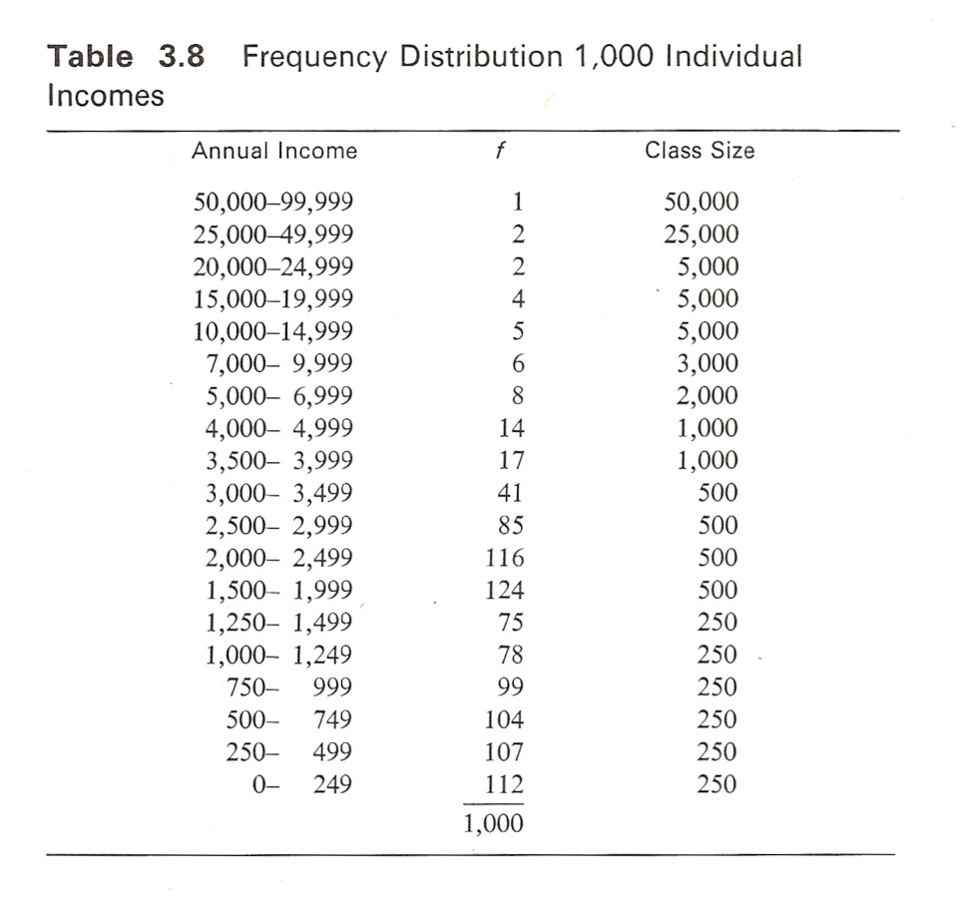
\includegraphics[width=4in]{Unequal_Income.png}
\caption{Unequal Income}
\end{figure}

\section{Relative Frequency
Distributions}\label{relative-frequency-distributions}

\begin{itemize}
\itemsep1pt\parskip0pt\parsep0pt
\item
  These are frequency distributions with proportion or percentage of
  each class interval
\item
  Useful for comparisons of two or more groups especially when the
  number in each group differ
\end{itemize}

\section{Relative Frequency Distribution
Example}\label{relative-frequency-distribution-example}
\vspace{2in} 

\section{Relative Frequency by
Groups}\label{relative-frequency-by-groups}

\begin{verbatim}
##     
##               PG   R
##     [10, 25)   0   1
##     [25, 40)   0   1
##     [40, 55)   0   0
##     [55, 70)   1   0
##     [70, 85)   3  10
##    [85, 100)  23 111
##   [100, 115)   7  40
##   [115, 130)   5  21
##   [130, 145)   3   8
##   [145, 160)   0   2
##   [160, 175)   0   1
\end{verbatim}

\section{Cumulative Frequency
Distributions}\label{cumulative-frequency-distributions}
\vspace{2in} 

\section{Cumulative Frequency
Creation}\label{cumulative-frequency-creation}

\begin{enumerate}
\def\labelenumi{\arabic{enumi}.}
\itemsep1pt\parskip0pt\parsep0pt
\item
  Start with a basic frequency distribution, grouped or ungrouped.
\item
  Starting with the smallest value, keep a running tally of the number
  encountered.

  \begin{itemize}
  \itemsep1pt\parskip0pt\parsep0pt
  \item
    This can be done by taking the frequency for the current category
    plus all prior categories
  \end{itemize}
\item
  Optional - add columns for cumulative proportion or cumulative
  percentage.
\end{enumerate}

\section{Frequency Distribution for Qualitative
Variables}\label{frequency-distribution-for-qualitative-variables}

\begin{verbatim}
## 
##       NC-17    PG PG-13     R 
## 53864    16   528  1003  3377
\end{verbatim}

\section{Graphs}\label{graphs}

\begin{itemize}
\itemsep1pt\parskip0pt\parsep0pt
\item
  Graphs are a great alternative to many of the tables we discussed
  above as they tend to be easier to quickly interpret and understand.
\item
  One benefit of graphs is the ability to explore the shape of
  distributions.
\item
  However, it is also easier to create misleading graphics.
\item
  Graphs for quantiative variables:

  \begin{itemize}
  \itemsep1pt\parskip0pt\parsep0pt
  \item
    Histograms
  \item
    Frequency Polygons
  \item
    Cumulative Polygon (Ogive)
  \item
    Stem and Leaf
  \end{itemize}
\item
  Graphs for qualitative variables:

  \begin{itemize}
  \itemsep1pt\parskip0pt\parsep0pt
  \item
    Bar Graphs
  \item
    Pie Charts
  \end{itemize}
\item
  Note: there are many other graphs that can be used too that we are not
  discussing.
\end{itemize}

\section{Histograms}\label{histograms}

\begin{itemize}
\itemsep1pt\parskip0pt\parsep0pt
\item
  A histogram is a visual representation of a frequency table for
  quantitative variables.
\item
  No gaps between bars as the x-axis is continuous.
\end{itemize}

\begin{figure}[H]
\centering
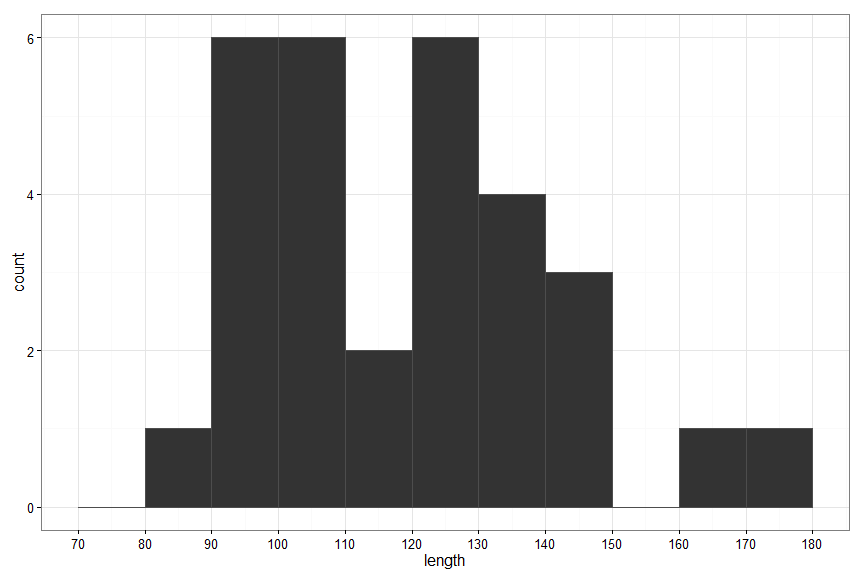
\includegraphics[width=4in]{figure/hist-1.png}
\caption{plot of chunk hist}
\end{figure}

\section{Shapes of Distributions}\label{shapes-of-distributions}

\begin{itemize}
\itemsep1pt\parskip0pt\parsep0pt
\item
  Distributions can be categorized based on their symmetry (skewness)
  and kurtosis.
\item
  Symmetry/Skewness is the amount a distribution leans one way or the
  other.

  \begin{itemize}
  \itemsep1pt\parskip0pt\parsep0pt
  \item
    A symmetric distribution is one where each half of the distribution
    are mirror images of one another.
  \item
    An asymmetric (skewed) distribution is one where they are not mirror
    images.
  \item
    A positively (right) skewed distribution is one where the bulk of
    data lie in the lower portion with a long upper tail.
  \item
    A negatively (left) skewed distribution is one where the bulk of
    data lie in the upper portion with a long lower tail.
  \end{itemize}
\item
  Kurtosis refers to the peakedness of the distribution. Relatedly, this
  also refers to the portion of the distribution that resides in the
  tails.

  \begin{itemize}
  \itemsep1pt\parskip0pt\parsep0pt
  \item
    Mesokurtic refers to an intermediate distribution with average tails
    and peakedness.
  \item
    Platykurtic refers to a distribution that is flatter with more
    observations in the tail.
  \item
    Leptokurtic refers to a distribution that is steeper with fewer
    observations in the tail.
  \end{itemize}
\end{itemize}

\section{Describing Distributions}\label{describing-distributions}

\begin{itemize}
\itemsep1pt\parskip0pt\parsep0pt
\item
  Location (Central Tendency)

  \begin{itemize}
  \itemsep1pt\parskip0pt\parsep0pt
  \item
    Where is the middle score?
  \item
    Where are the scores concentrated?
  \end{itemize}
\item
  Variability

  \begin{itemize}
  \itemsep1pt\parskip0pt\parsep0pt
  \item
    Dispersion
  \item
    Spread
  \item
    Range
  \end{itemize}
\end{itemize}

\section{Examples of common shapes}\label{examples-of-common-shapes}

\begin{figure}[H]
\centering
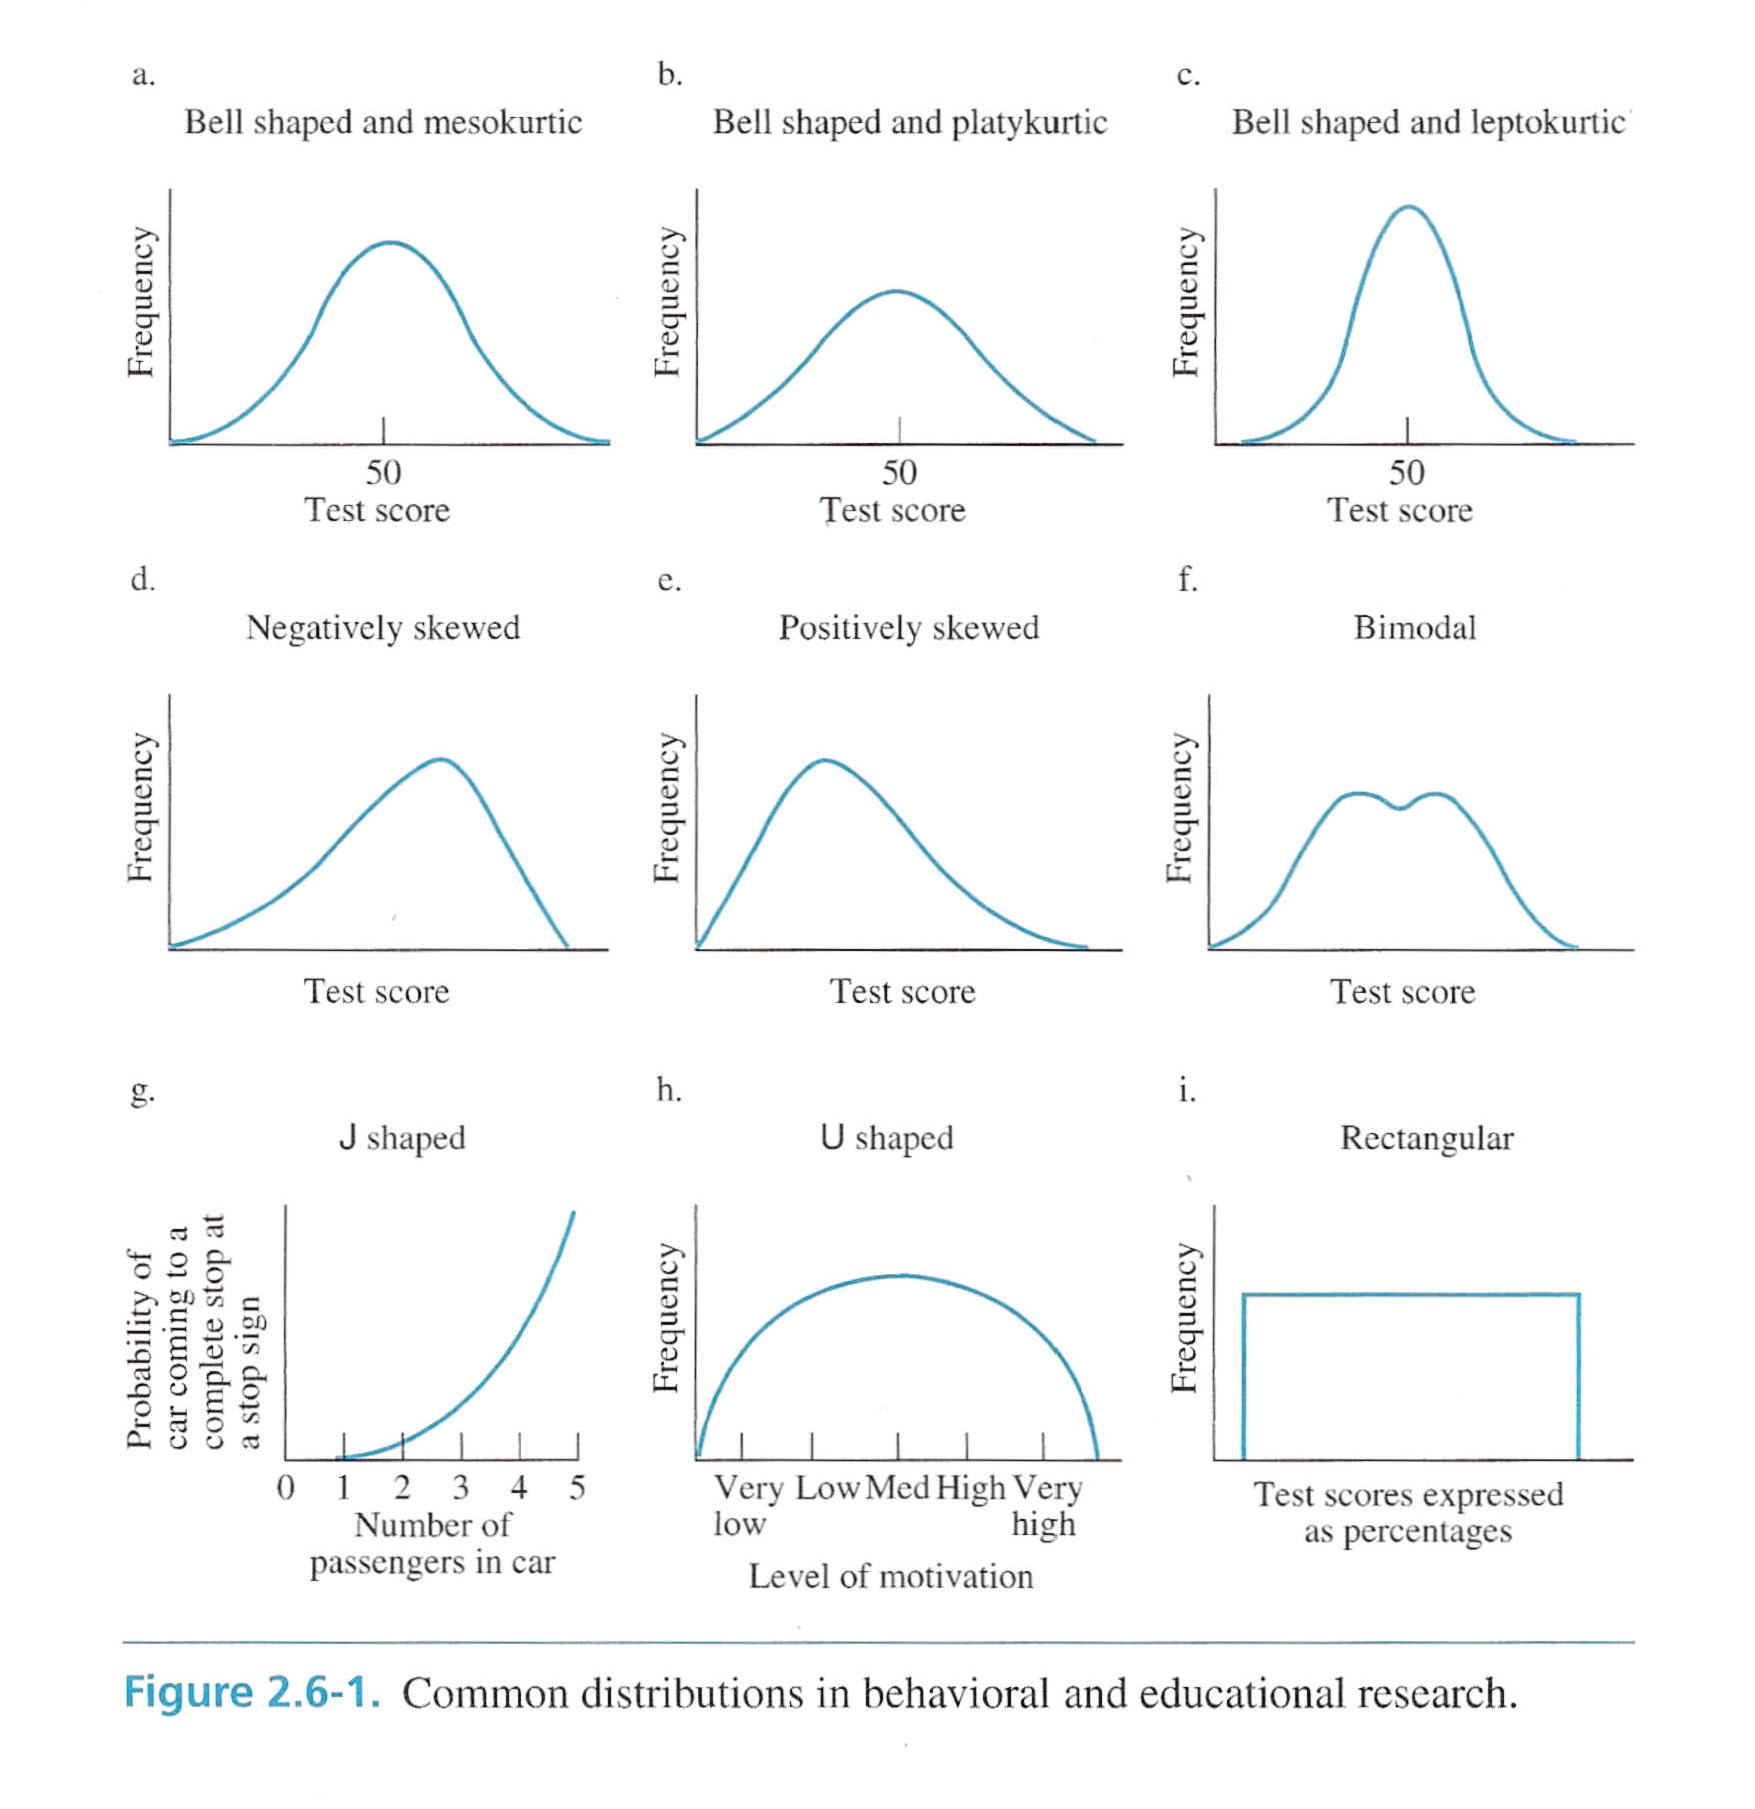
\includegraphics[width=4in]{Dist_shape.png}
\caption{Distribution Shapes}
\end{figure}

\section{Shapes with Histograms}\label{shapes-with-histograms}

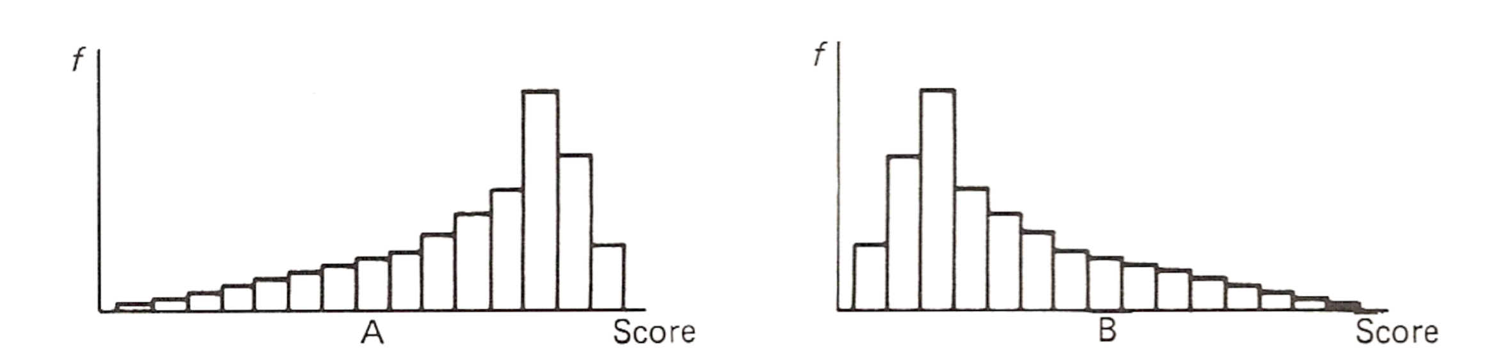
\includegraphics[width=4in]{skew_dist.png} \\
 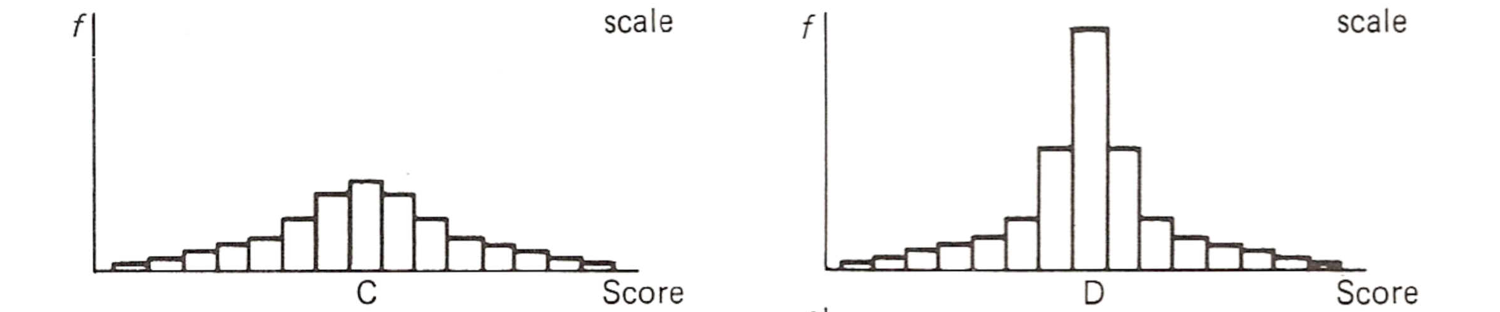
\includegraphics[width=4in]{kurt_dist.png}

\section{Factors Affecting Distribution
Shape}\label{factors-affecting-distribution-shape}

\begin{enumerate}
\def\labelenumi{\arabic{enumi}.}
\itemsep1pt\parskip0pt\parsep0pt
\item
  Sampling

  \begin{itemize}
  \itemsep1pt\parskip0pt\parsep0pt
  \item
    The larger the sample size, the closer it will approximate the
    population.
  \end{itemize}
\item
  Relative Scale

  \begin{itemize}
  \itemsep1pt\parskip0pt\parsep0pt
  \item
    The height of the histogram should be 3/4 of the width.
  \end{itemize}
\item
  Frequency Scale

  \begin{itemize}
  \itemsep1pt\parskip0pt\parsep0pt
  \item
    Always continuous and start at 0.
  \end{itemize}
\item
  Interval size / number of intervals
\end{enumerate}

\section{Effect of Sampling}\label{effect-of-sampling}

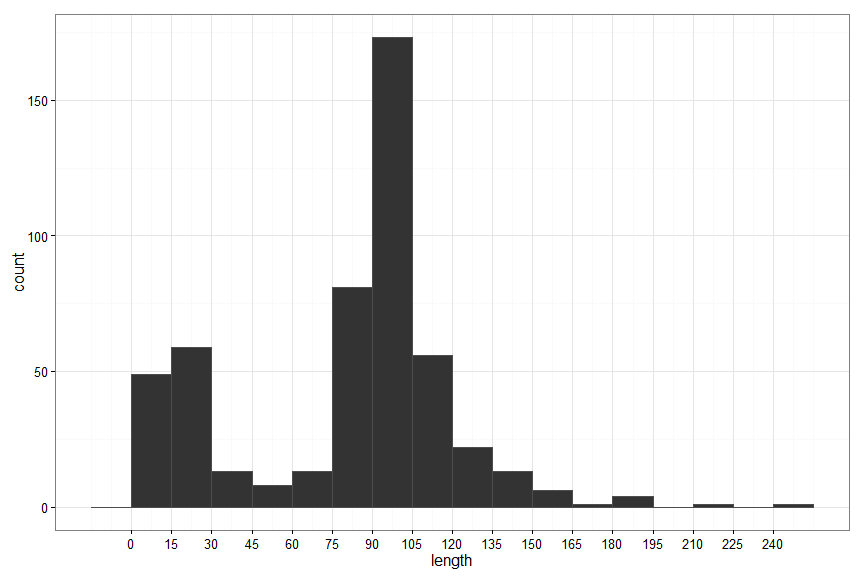
\includegraphics[width=3.5in]{figure/histsamp-1.png}
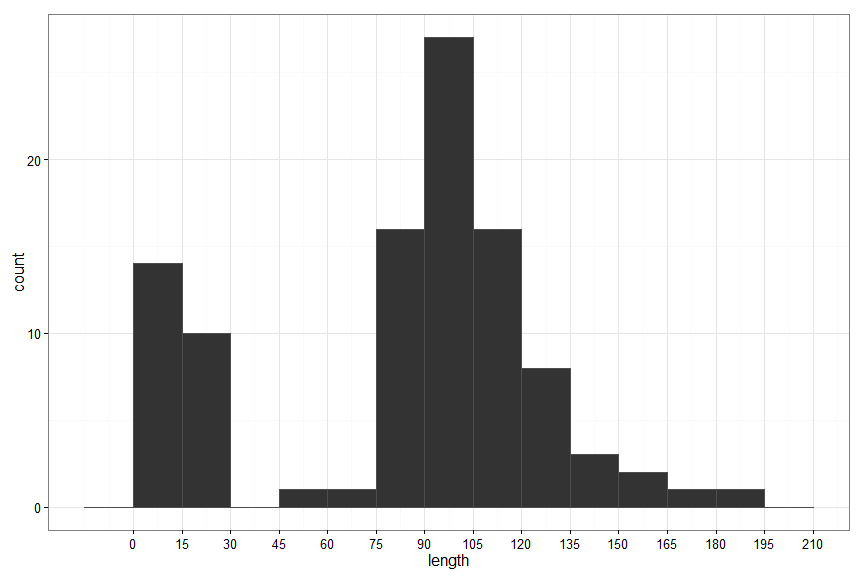
\includegraphics[width=3.5in]{figure/histsamp-2.png}\\
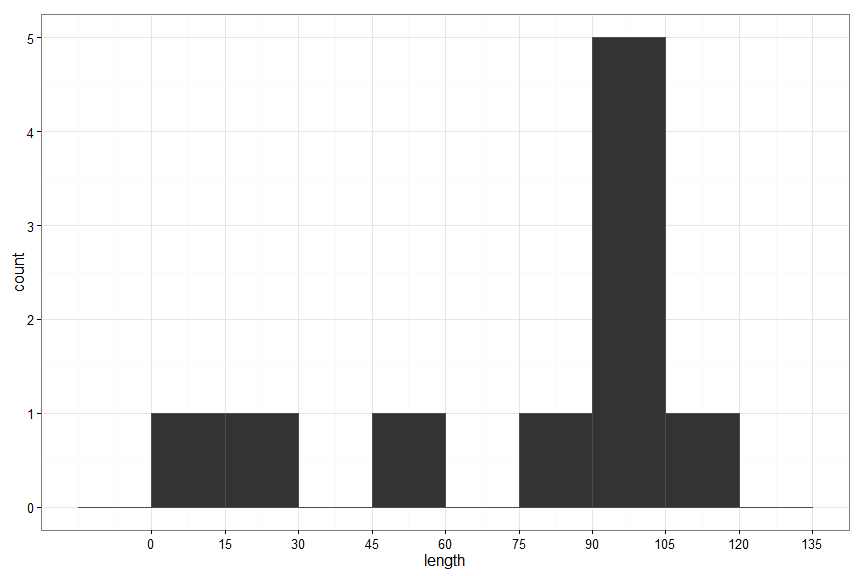
\includegraphics[width=3.5in]{figure/histsamp-3.png}

\section{Effect of Relative Scale}\label{effect-of-relative-scale}

\begin{figure}[H]
\centering
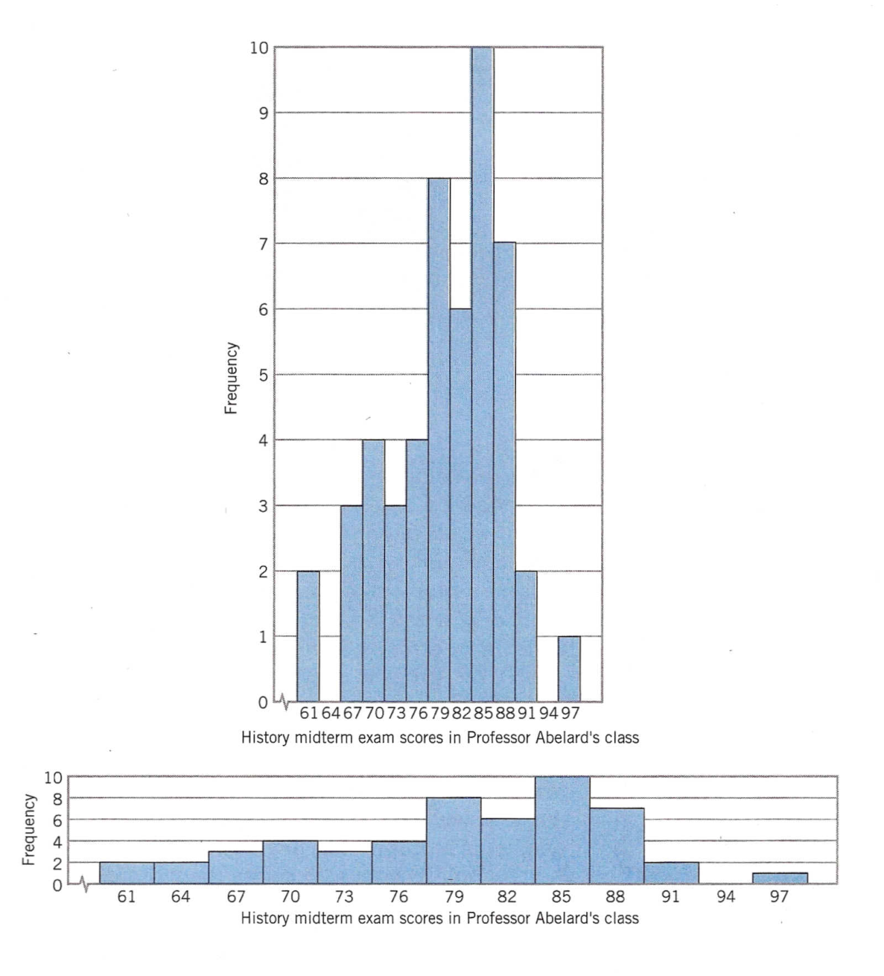
\includegraphics[width=4in]{Relative_Scale.png}
\caption{Relative Scale}
\end{figure}

\section{Effect of Frequency Not Starting at
Zero}\label{effect-of-frequency-not-starting-at-zero}

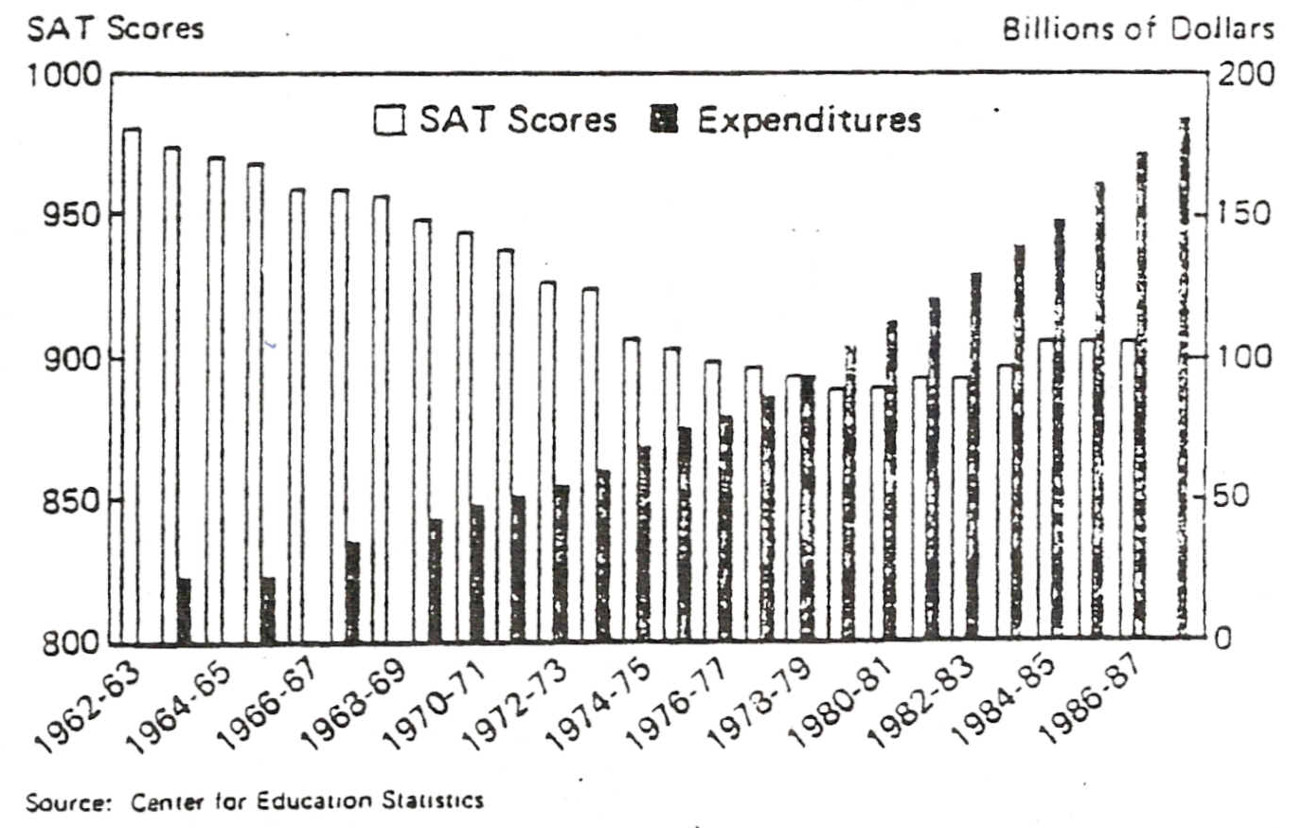
\includegraphics[width=3.5in]{Freq_NotZero.png}
 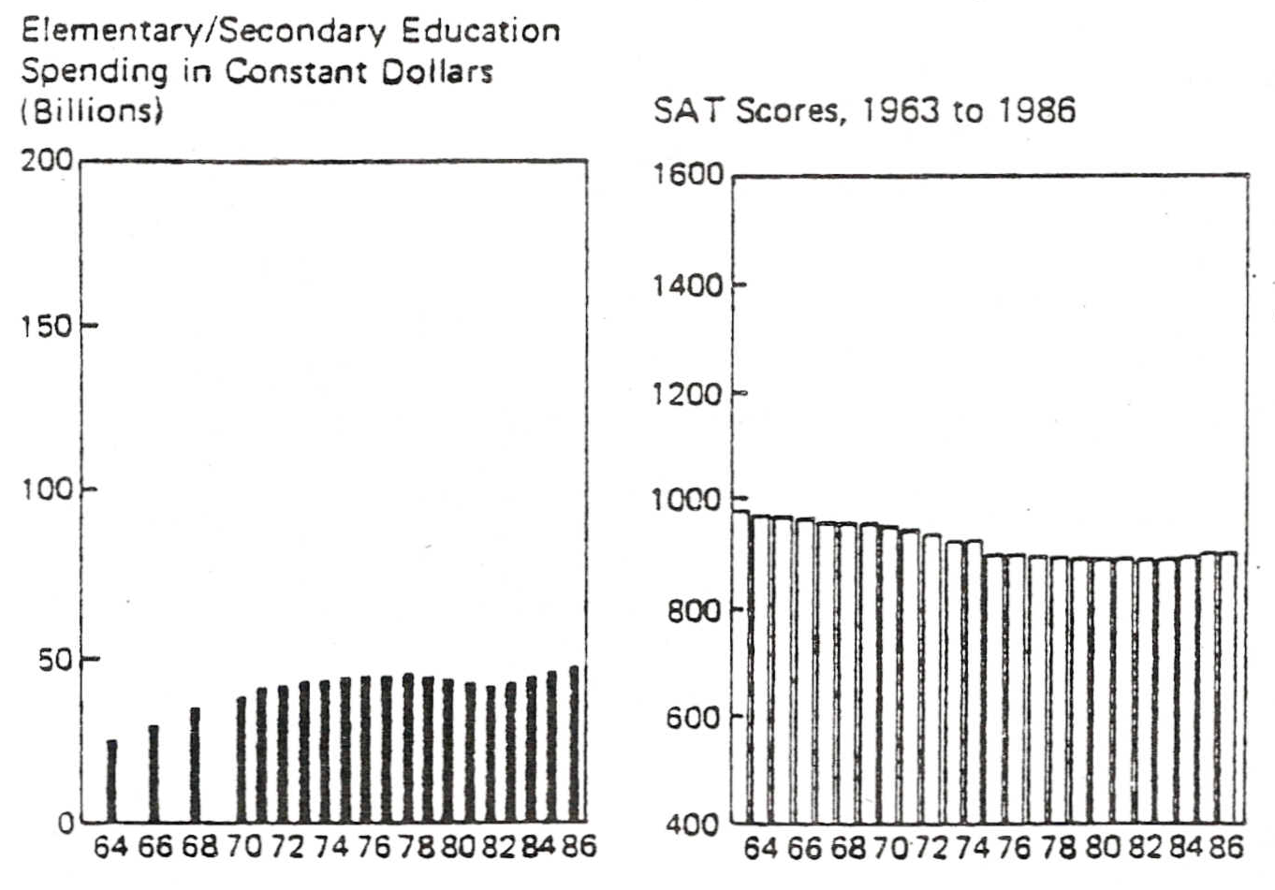
\includegraphics[width=3.5in]{Freq_NotZero2.png}

\section{Effect of Binwidth on
Histograms}\label{effect-of-binwidth-on-histograms}

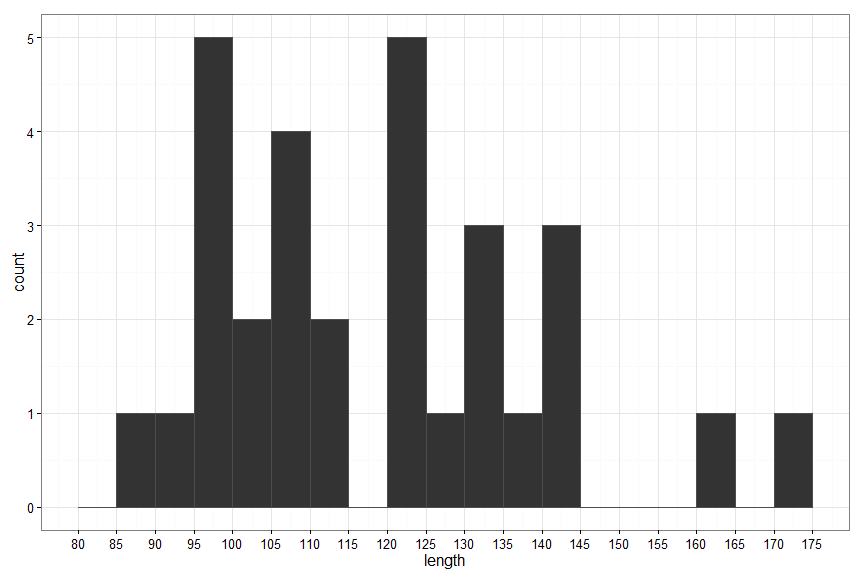
\includegraphics[width=3.5in]{figure/histbin-1.png}
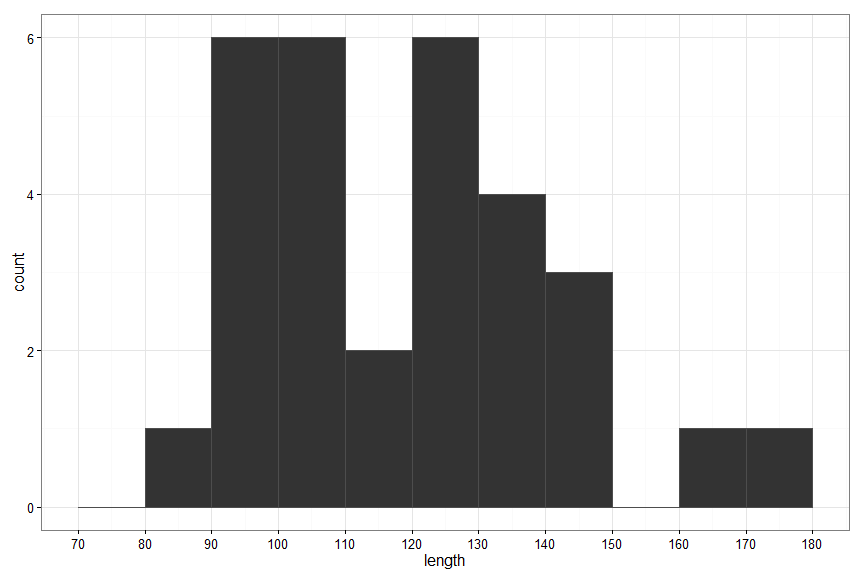
\includegraphics[width=3.5in]{figure/histbin-2.png}\\
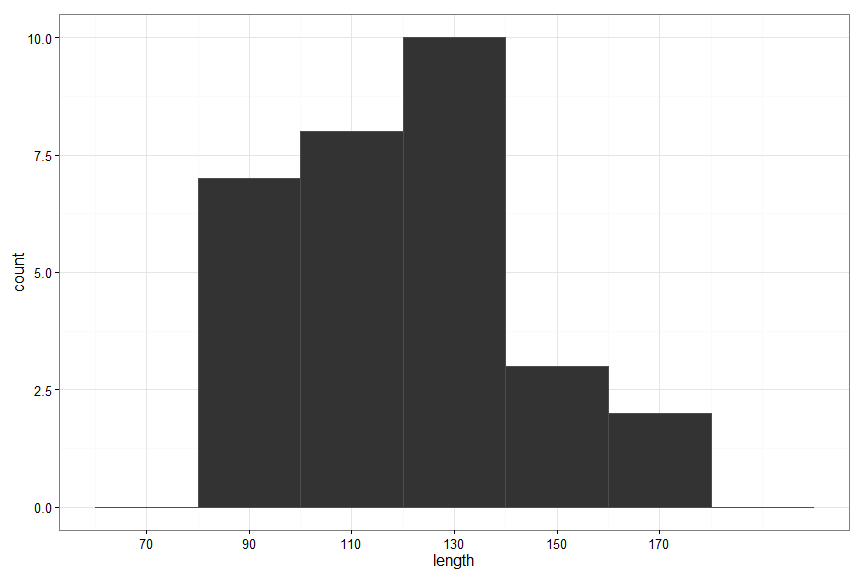
\includegraphics[width=3.5in]{figure/histbin-3.png}
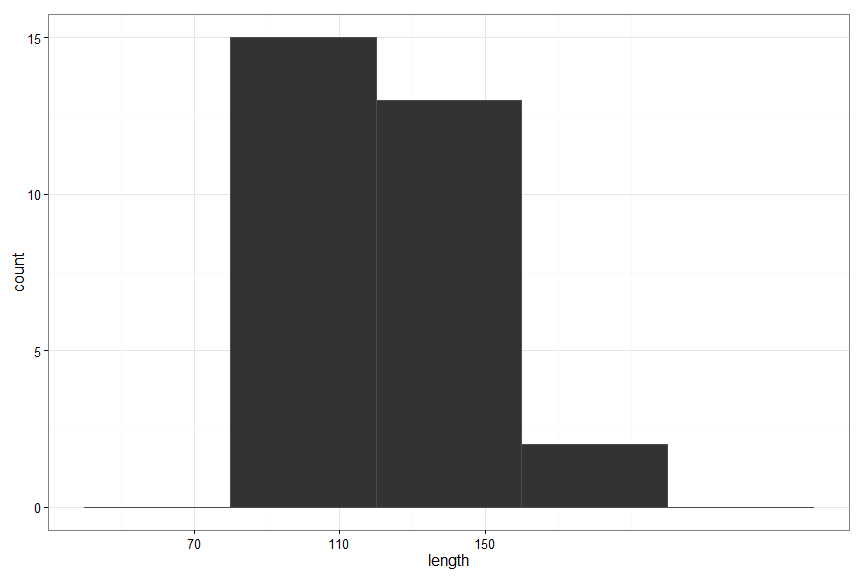
\includegraphics[width=3.5in]{figure/histbin-4.png}

\section{Cumulative Polygon (Ogive)}\label{cumulative-polygon-ogive}

\begin{itemize}
\itemsep1pt\parskip0pt\parsep0pt
\item
  The cumulative polygon or ogive, is a graphical representation of the
  cumulative frequency.
\item
  This plot is unique in that it never decreases.
\end{itemize}

\begin{figure}[H]
\centering
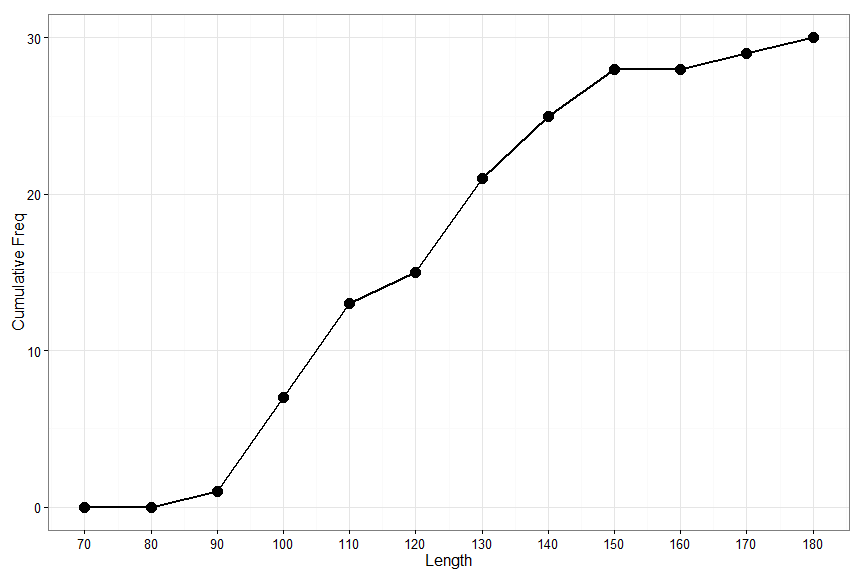
\includegraphics[width=4in]{figure/ogive-1.png}
\caption{plot of chunk ogive}
\end{figure}

\section{Ogive - Cumulative
Percentage}\label{ogive---cumulative-percentage}

\begin{figure}[H]
\centering
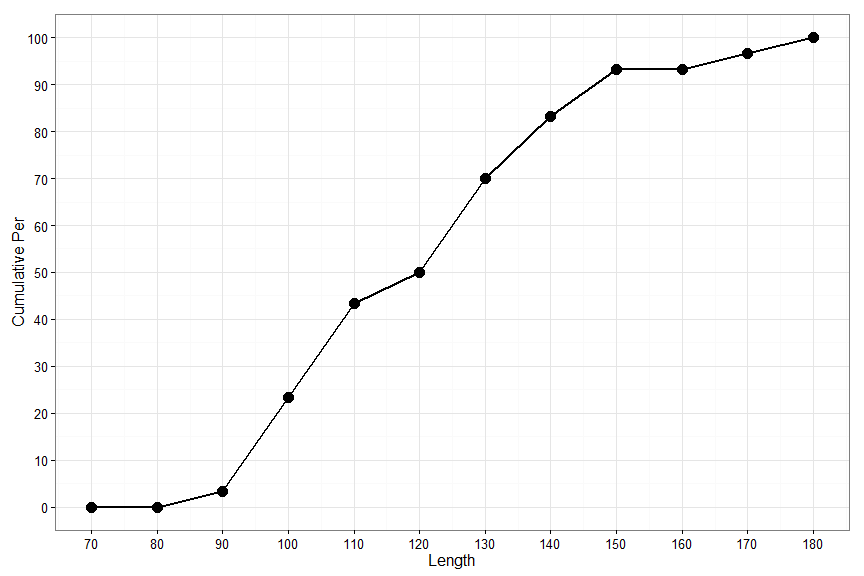
\includegraphics[width=4in]{figure/ogivepercent-1.png}
\caption{plot of chunk ogivepercent}
\end{figure}

\section{Real Life Ogive Example}\label{real-life-ogive-example}

\begin{figure}[H]
\centering
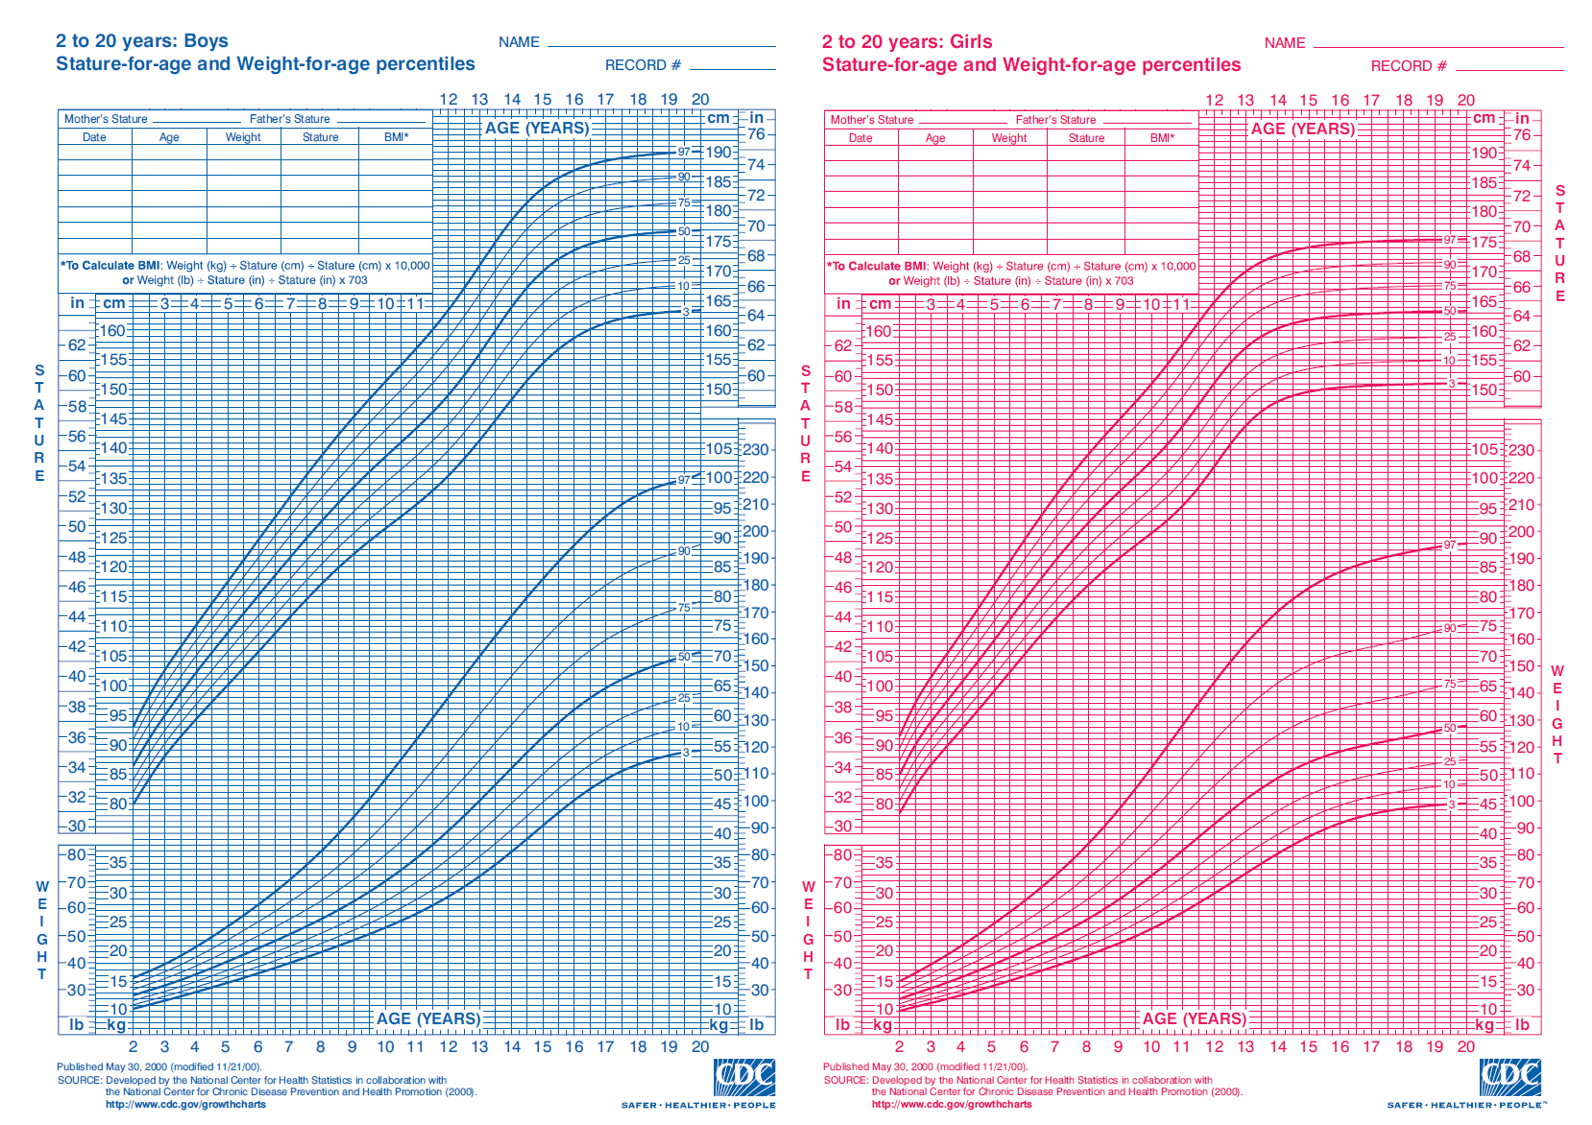
\includegraphics[width=4in]{Ogive_Examp.png}
\caption{Ogive Examp}
\end{figure}

\section{Percentile Ranks and
Percentiles}\label{percentile-ranks-and-percentiles}

\begin{itemize}
\itemsep1pt\parskip0pt\parsep0pt
\item
  Percentile Ranks:

  \begin{itemize}
  \itemsep1pt\parskip0pt\parsep0pt
  \item
    The percentage of scores at or below a given point.
  \item
    Denoted by \(P_{R}(X)\), read as the percentile rank of score \(X\).
  \end{itemize}
\item
  Percentiles:

  \begin{itemize}
  \itemsep1pt\parskip0pt\parsep0pt
  \item
    The point on the score scale below which a specified percentage of
    scores fall.
  \item
    Denoted by $P_{\%}\%$
  \end{itemize}
\item
  A percentile is the inverse of a percentile rank.
\item
  The percentile rank of a given point on the score scale is the
  percentage of scores falling below this point in the ordered series of
  scores.

  \begin{itemize}
  \itemsep1pt\parskip0pt\parsep0pt
  \item
    The value of the point iteself is the percentile corresponding to
    this percentile rank.
  \item
    Example: if \(P_{R}(X) = 60\), then \(P_{60} = X\).
  \end{itemize}
\item
  Never say, `My score was \textbf{in} the top quartile'.

  \begin{itemize}
  \itemsep1pt\parskip0pt\parsep0pt
  \item
    A quartile (or percentile or decile) is a point on the score scale,
    not an interval.
  \item
    Instead say, `My score was at the top quartile'.
  \end{itemize}
\end{itemize}

\section{Special Percentile Points}\label{special-percentile-points}

\begin{itemize}
\itemsep1pt\parskip0pt\parsep0pt
\item
  Deciles:

  \begin{itemize}
  \itemsep1pt\parskip0pt\parsep0pt
  \item
    \(D_{1} = P_{10}\) - First decile
  \item
    \(D_{2} = P_{20}\) - Second decile
  \item
    \(D_{5} = Q_{2} = P_{50} = Mdn\) - Median
  \item
    \(Q_{1} = P_{25}\) - First Quartile
  \item
    \(Q_{3} = P_{75}\) - Third Quartile
  \end{itemize}
\end{itemize}

\section{Estimate Percentile
Ranks/Percentiles}\label{estimate-percentile-rankspercentiles}

\begin{figure}[H]
\centering
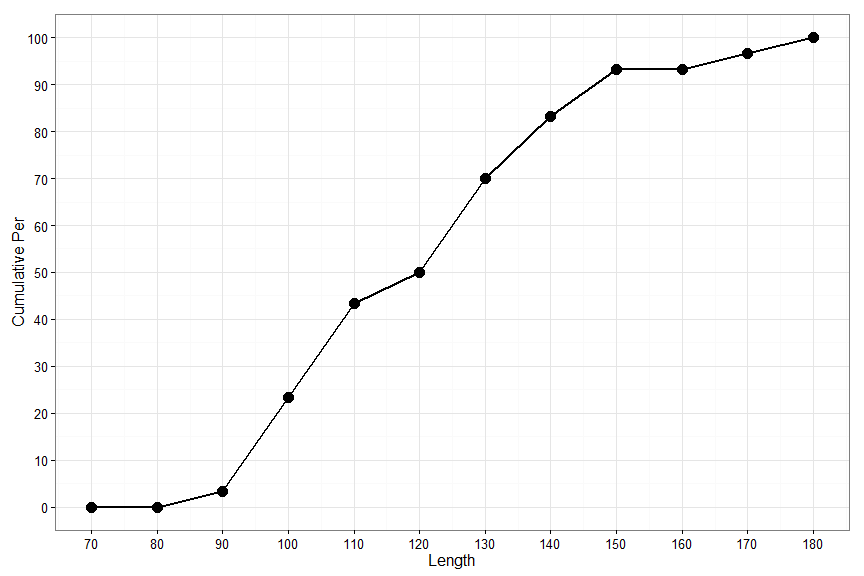
\includegraphics[width=4in]{figure/ogivepercent2-1.png}
\caption{plot of chunk ogivepercent2}
\end{figure}

\begin{itemize}
\itemsep1pt\parskip0pt\parsep0pt
\item
  $P_{R}(122) = $
\item
  $P_{R}(160) = $
\item
  $P_{50} = $
\item
  $P_{80} = $
\end{itemize}

\section{Decile Differences}\label{decile-differences}

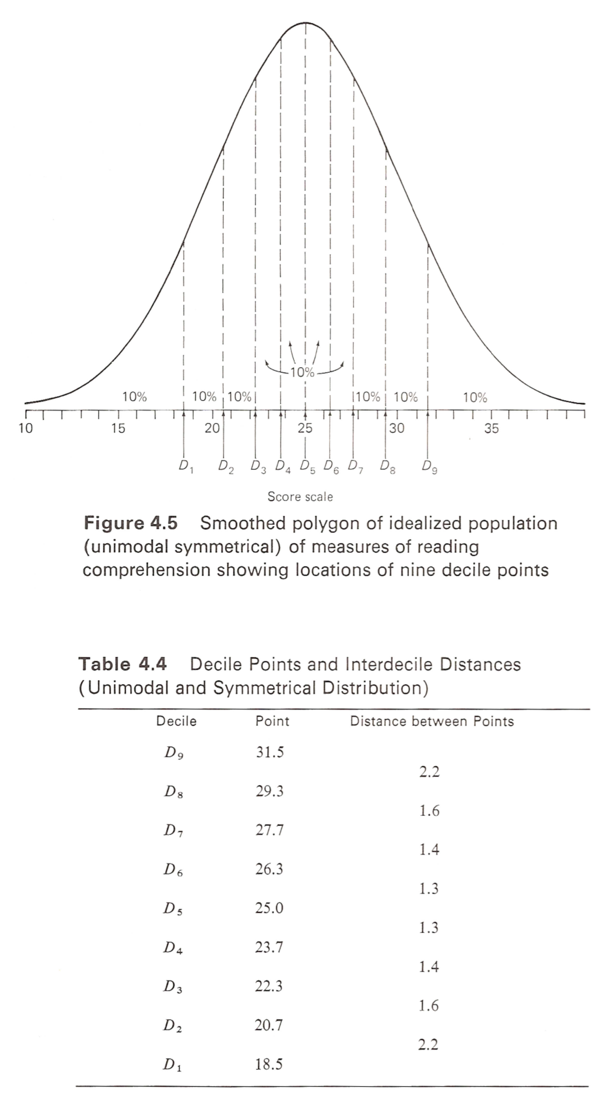
\includegraphics[width=3.5in]{Decile_Normal.png}
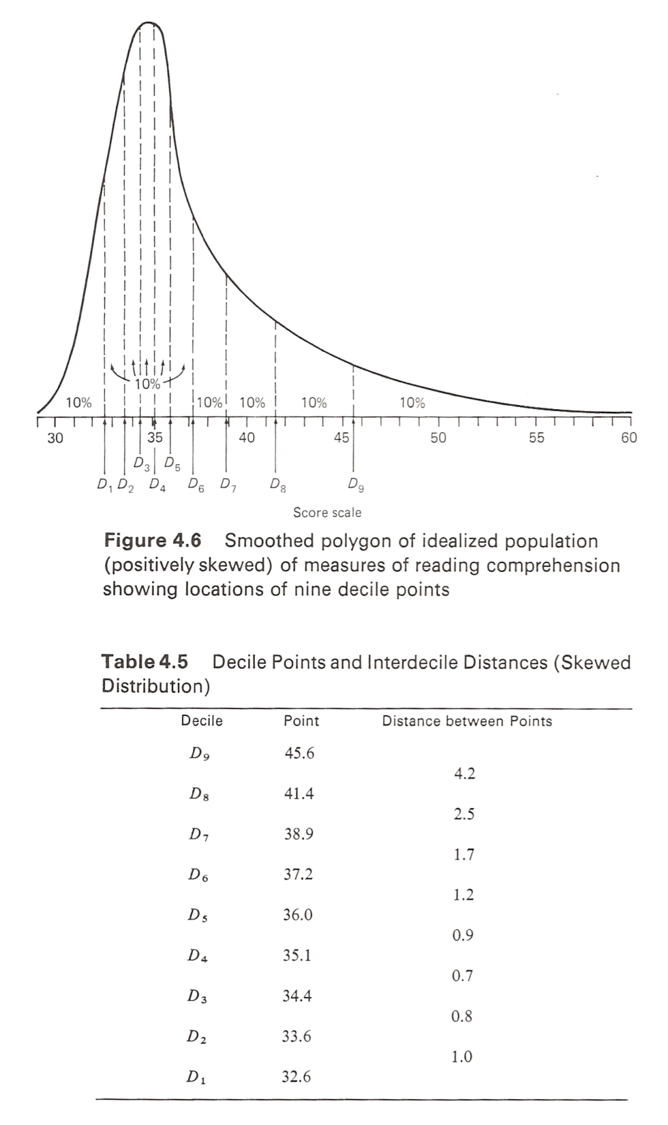
\includegraphics[width=3.5in]{Decile_Skew.png}\\
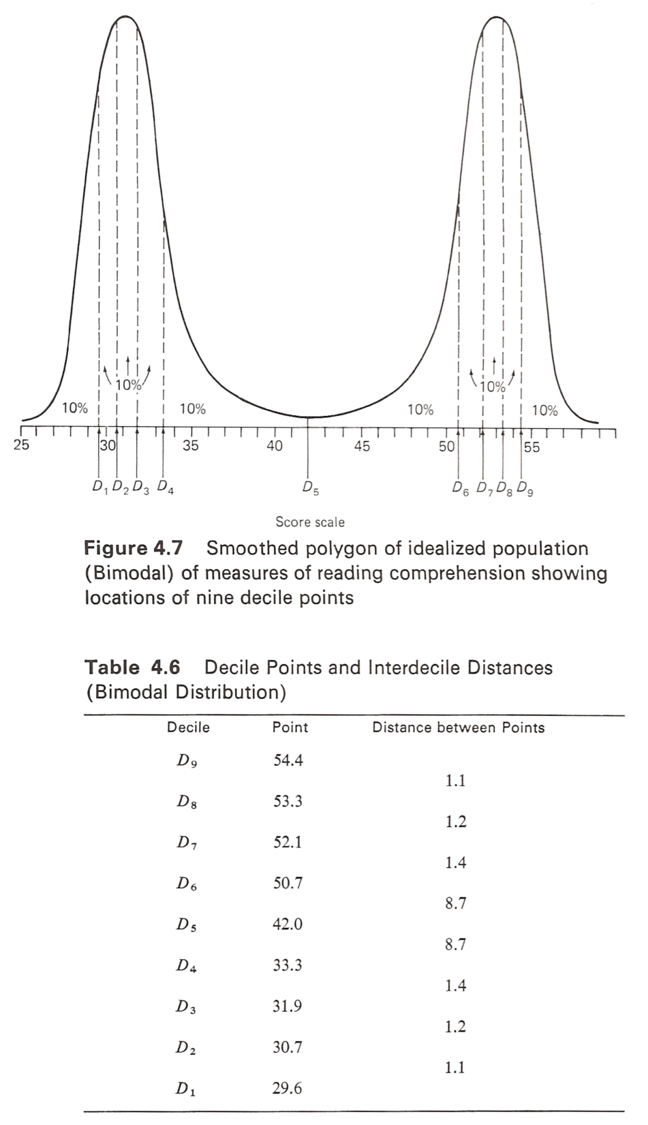
\includegraphics[width=4in]{Decile_Bimodal.png}

\section{Quartiles and Shape}\label{quartiles-and-shape}

\begin{itemize}
\itemsep1pt\parskip0pt\parsep0pt
\item
  Symmetrical:

  \begin{itemize}
  \itemsep1pt\parskip0pt\parsep0pt
  \item
    \(Q_{3} - Q_{2} = Q_{2} - Q_{1}\)
  \end{itemize}
\item
  Positive Skew:

  \begin{itemize}
  \itemsep1pt\parskip0pt\parsep0pt
  \item
    \(Q_{3} - Q_{2} > Q_{2} - Q_{1}\)
  \end{itemize}
\item
  Negative Skew:

  \begin{itemize}
  \itemsep1pt\parskip0pt\parsep0pt
  \item
    \(Q_{3} - Q_{1} < Q_{2} - Q_{1}\)
  \end{itemize}
\end{itemize}

\section{Ogive Shape}\label{ogive-shape}

\begin{figure}[H]
\centering
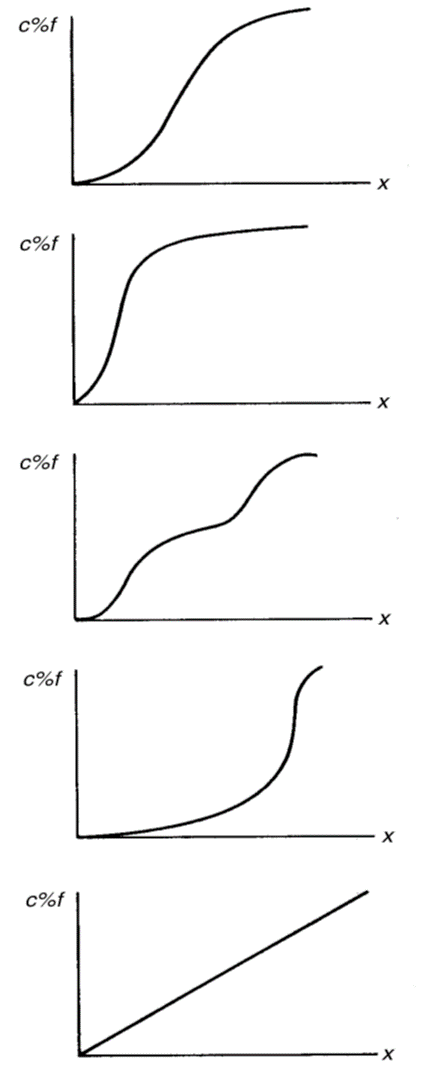
\includegraphics[width=4in]{Ogive_Shape.png}
\caption{Ogive Shape}
\end{figure}

\section{Calculating Percentiles and Percentile
Ranks}\label{calculating-percentiles-and-percentile-ranks}

\begin{itemize}
\itemsep1pt\parskip0pt\parsep0pt
\item
  Percentiles:

  \begin{itemize}
  \itemsep1pt\parskip0pt\parsep0pt
  \item
    $ P_{\%} = X_{ll} + i
    \left(\frac{n(\frac{P_{R}}{100}) - \sum f_{b}}{f_{i}}\right) $
  \end{itemize}
\item
  Percentile Ranks

  \begin{itemize}
  \itemsep1pt\parskip0pt\parsep0pt
  \item
    $ P_{R}(X) = \frac{100}{n}\left(\sum f_{b} +
    \frac{f_{i}(P_{\%} - X_{ll})}{i}\right)$  
    \\
 where:
  \item
    X = Score of Interest
  \item
    n = Total Sample size
  \item
    \(\sum f_{b}\) = Number of scores below interval containing X
  \item
    i = interval size = \(X_{ul} - X_{ll}\)
  \item
    \(X_{ll}\) = Lower limit of interval containing X
  \item
    \(X_{ul}\) = Upper limit of interval containing X
  \item 
     \(f_{i} \) = Number of observations within category.
  \end{itemize}
\end{itemize}

\section{Calculating Examples}\label{calculating-examples}

\begin{itemize}
\itemsep1pt\parskip0pt\parsep0pt
\item
  Using the table below, find \(P_{R}(112)\), \(P_{R}(158)\),
  \(P_{25}\), \(P_{50}\), \(P_{75}\)
\end{itemize}

\begin{verbatim}
##           freq cf
##              0  0
## [70,80)      0  0
## [80,90)      1  1
## [90,100)     6  7
## [100,110)    6 13
## [110,120)    2 15
## [120,130)    6 21
## [130,140)    4 25
## [140,150)    3 28
## [150,160)    0 28
## [160,170)    1 29
## [170,180)    1 30
\end{verbatim}

\section{Bar Graphs}\label{bar-graphs}

\begin{itemize}
\itemsep1pt\parskip0pt\parsep0pt
\item
  Bar graphs are a way to visually show a frequency table for
  qualitative variables.
\item
  Can also be used to show other variables on the y-axis for qualitative
  variables.
\item
  Has gaps to show the differences in groups.
\item
  Order should be meaningful, either alphabetical for nominal variables
  or in the correct order for ordinal variables.
\end{itemize}

\begin{figure}[H]
\centering
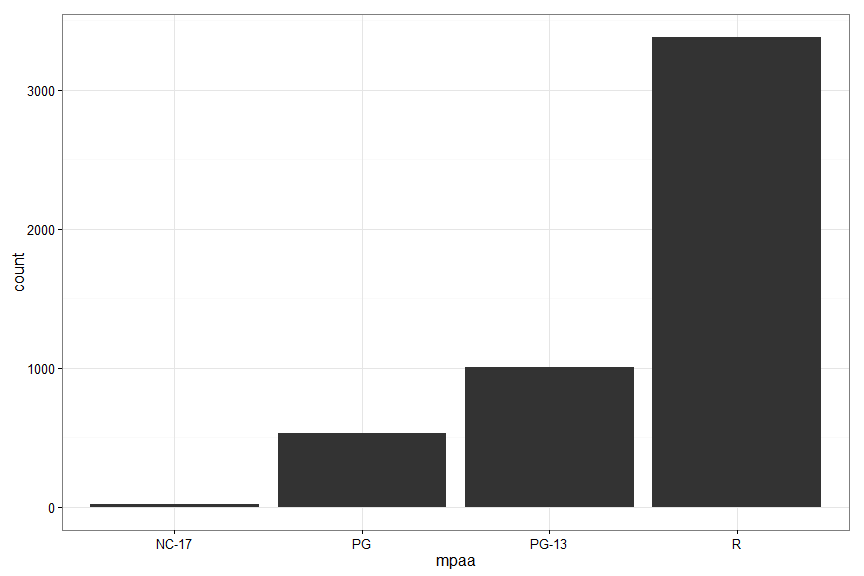
\includegraphics[width=4in]{figure/bar-1.png}
\caption{plot of chunk bar}
\end{figure}

\section{Pie Charts}\label{pie-charts}

\begin{itemize}
\itemsep1pt\parskip0pt\parsep0pt
\item
  Pie charts are useful to show the percentage of the whole for each
  group.
\item
  The sum of the pieces of the pie must add up to 100\% for this chart
  to be meaningful.
\end{itemize}

\begin{figure}[H]
\centering
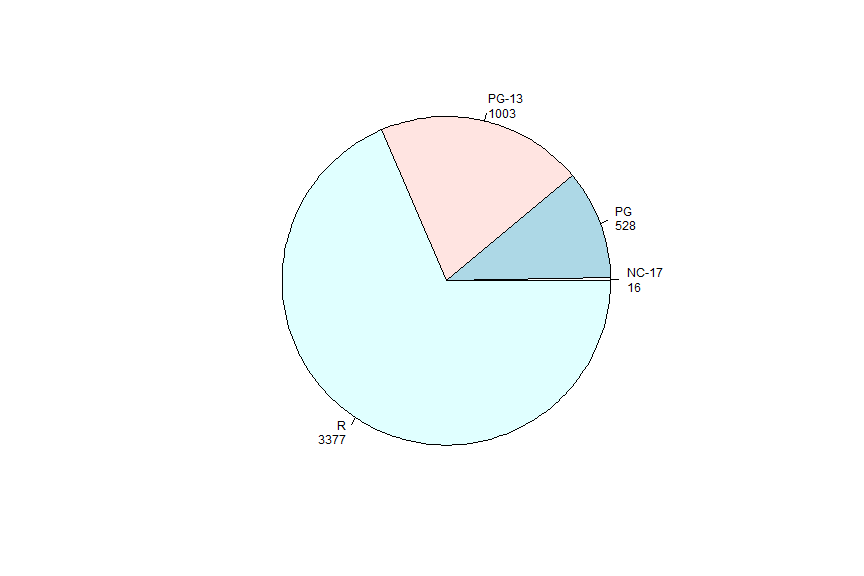
\includegraphics[width=4in]{figure/pie-1.png}
\caption{plot of chunk pie}
\end{figure}

\section{Poor graphics}\label{poor-graphics}

\begin{itemize}
\itemsep1pt\parskip0pt\parsep0pt
\item
  Care needs to be made when constructing good graphics.
\item
  It is easy for graphs to mislead/mask the purpose.
\item
  The goal should be to easily convey the message.
\end{itemize}

\href{http://flowingdata.com/2013/07/15/open-thread-what-is-wrong-with-these-charts/}{Poor
Charts}

\section{Interesting Graphic
Examples}\label{interesting-graphic-examples}

\href{http://www.washingtonpost.com/wp-srv/special/national/us-language-map/}{Languages
other than English Spoken at home}

\href{http://www.coopercenter.org/demographics/Racial-Dot-Map}{The
Racial Dot Map}

\end{document}
